\paragraph{Motivation}
Remote sensing has been an essential means of monitoring dynamic changes such as rainfall, wind, temperature, et al. for weather monitoring and disaster forecast.

Although water quality remains an essential element for the survival of flora and fauna, it is still monitored through in-situ monitoring stations. Even though these stations provide accurate data, their temporal and spatial resolution is inadequate. Thus, there is an opening
for satellite remote sensing to develop a method to monitor water quality.

\begin{minipage}{0.5\textwidth}
    One such parameter for monitoring water quality is dissolved oxygen, which is defined as the amount of free and non-compound oxygen dissolved in the water body(Chi et al., 2020). Monitoring DO can help us predict changes in that marine ecosystem and implement remedies, considering that even a minor change can cause a significant negative impact.
    
    \paragraph*{}
    Literature such as Keeling et al., 2010\cite{keeling_2010} suggests that dissolved oxygen in the open ocean has been declining in the past centuries due to natural causes or increased temperature or changes in salinity.
\end{minipage}
\begin{minipage}{0.5\textwidth}
    \begin{figure}[H]
        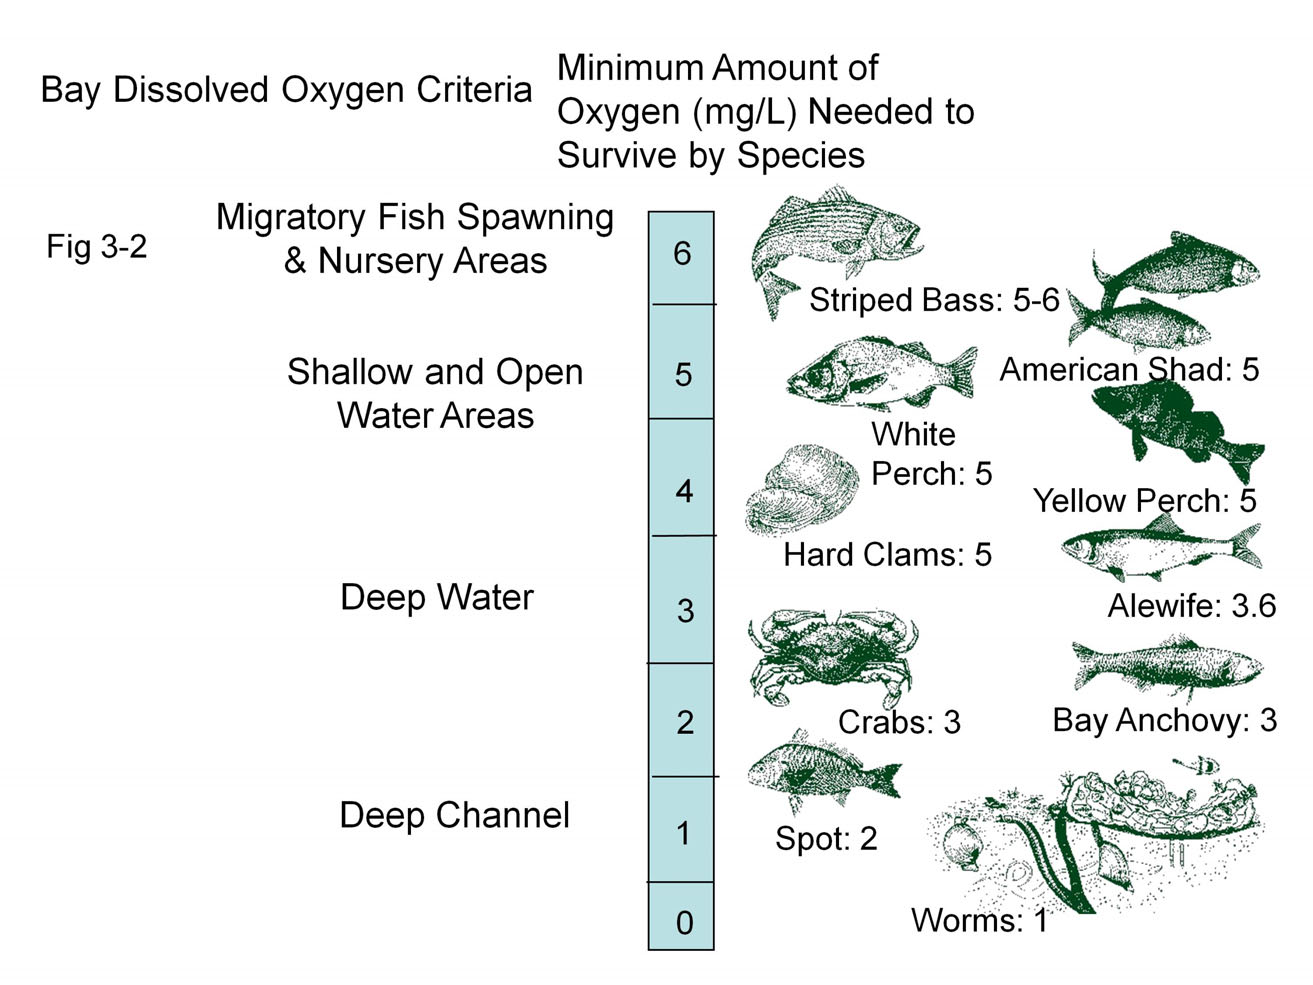
\includegraphics[height=5cm]{figs/fish_requirements.jpg}
        \caption{Requirement of DO for marine life}
    \end{figure}
\end{minipage}



DO decreases exponentially with the increase in salinity(Chi et al., 2020).

In summer and winter, the temperature differential is small between day and night, affecting the convection process and hampering the mixture of upper and lower layers of the ocean; due to this and continuous consumption of DO in the lower layers can lead to hypoxic situations.
The temperature differential is high in spring and autumn between day and night, allowing the layers to mix and keep the DO concentration consistent.

The traditional method of in-situ measurements is very time and labor-intensive, so this project aims to develop and verify a correlation between dissolved oxygen, temperature, salinity, and chlorophyll content.


% \paragraph*{}
%     Remote sensing has been an important means of monitoring dynamic changes such as rainfall, wind, temperature, etc patterns for weather monitoring and disaster forecast.

%     Dissolved oxygen(DO) is defined as the amount of free and non-compound oxygen dissolved in the water body(Chi et. al 2020)

%     Although, water quality remains an improtant element for the survial of flura and fauna, it is still monitored through in-situ monitoring stations; though, these stations provide accurate data there temporal and spatial resolution is inadquate. Hence, there is an opening
%     for satellite remote sensing to develop a method to monitor water quality.

%     One such parameter is dissolved oxygen, it is the amount of oxygen present in a water body. Water bodies receie oxygen from the atmosphere and from the aquatic plants with stagnant bodies having less content than moving ones.

%     Hence, we can extrapolate that dissolved oxygen is directly lines to the marine ecosystem and even a little change can cause a negative imapct.

%     Some literature such as Keeling et al.[2010] suggets that dissolved oxygen in open ocean has been declining in the past centuries, be it due to natural causes or increase in temperature.

%     The traditional method of in-situ measurements is very time and labour intensive, so the idea of this project is to develop and verify a correlation between dissolved oxygen, temperature, salinity, chlorophyll content.

%     Over the past severl decades, water quality retrieval by remote sensing has been widely concerned and developed rapidly (Dekker etal. 1992; Duan et al. 2012; Gons, 1999)

%     In existing research, the most focused water quality parameters include Chlorophyll-a, temperature and colored dissolved organic matter(CDM); other parameters which can be helpful for estimating dissolved oxygen are salinity, turbidity, nitrate concentration and specific conductance.


%     DO decreases expnentially with the increase in salinity(Chi et al. 2020).

%     In summer and winter, the temperature of upper layer of water body is relatively higher or lower than the lower layer(>3m) and the temperature differenece between day and night is small(Walker and Lucke, 2018). As a result the upper layer is less dense and remains at the top of the lake. The mixture of layers is cut-off but DO is consumed continuously in the lower layer which leads to DO decrease and even hypoix situations.

%     In spring and autumn, due to increas in the temperature variations, the density of upper layer is lower in daytime and higher in night, which promotes the mixture between the layers allowing the DO to remain consistant.
